% !TEX root = Document.tex
\Chapter{Choix de capteurs}\label{sec:capteurs}
%\color{red}
%Intégrer ce chapitre à la revue de littérature? Ou faire un chapitre très court.
%\color{black}

Il va de soit que pour qu'un robot puisse éviter des obstacles et se déplacer de façon autonome, il doit avoir un moyen de percevoir son environnement. Dans ce chapitre nous traitons des capteurs utilisables dans le contexte de la navigation de robots mobiles et possiblement de la reconstruction 3D. En général, il existe trois sortes de capteurs utilisés: la vision passive, la vision active et diverses sortes de télémètres.

\section{Systèmes passifs}

Dans la section \ref{subsec:stereo_vision} nous avons touché le sujet de vision stéréo, un exemple de premier plan d'un capteur passif c'est-à-dire un capteur capable de percevoir un phénomène quelconque sans devoir émettre un signal. En effet, les caméras sont un moyen peu coûteux de percevoir la profondeur et sont courramment utilisés dans des micro-véhicules aériens commerciaux tel que le Yuneec Typhoon H dans la Figure \ref{fig:yuneec}. Par contre, la vision stéréo n'étant pas infaillible, la perception de profondeur peut échouer dans les environnement comportant peu de texture ou trop peu de lumière. Malgré certaines méthodes de régularisation pour tenter de remplir les trous en propageant l'information des régions aux alentours \citep{Hirschmuller2008}, l'état de l'art est à un point où les entreprises jugent encore prudent d'ajouter un capteur secondaire, tel qu'un sonar dans la Figure \ref{subfig:yuneec_closeup}, pour compenser les échecs de perception.

\begin{figure}[ht]
  \centering
  \subfloat[]{
  	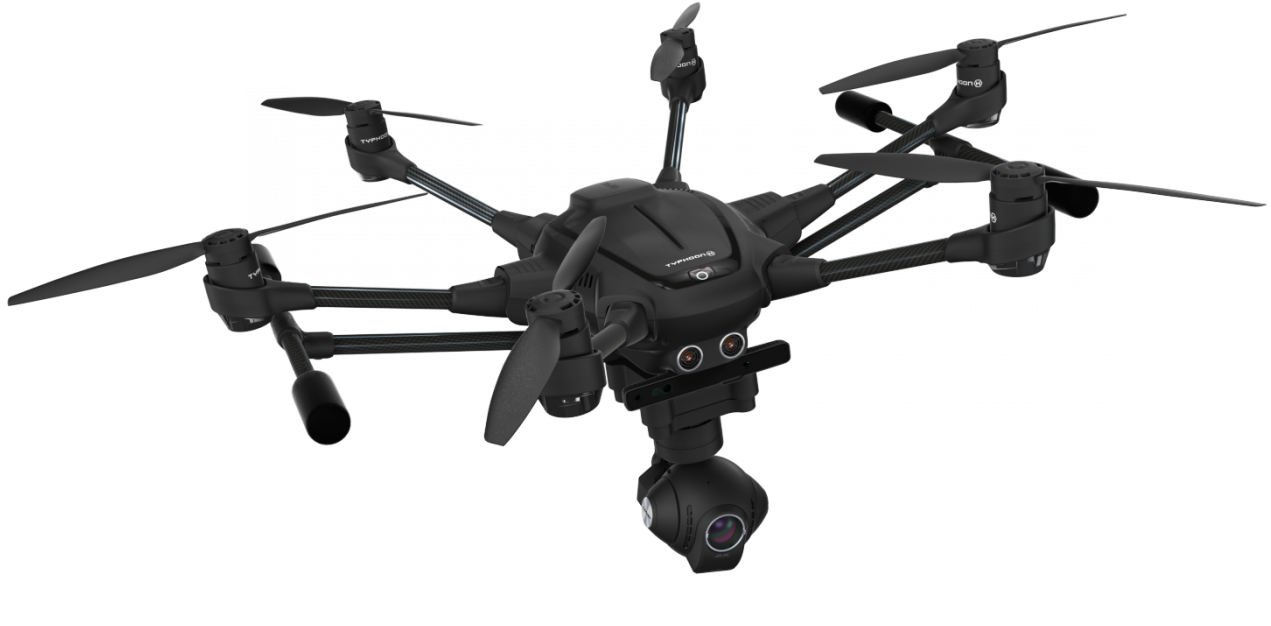
\includegraphics[width=0.60\linewidth]{images/yuneec_full.png}
  	\label{subfig:yuneec_full}
  }
  \hfil
  \subfloat[]{
  	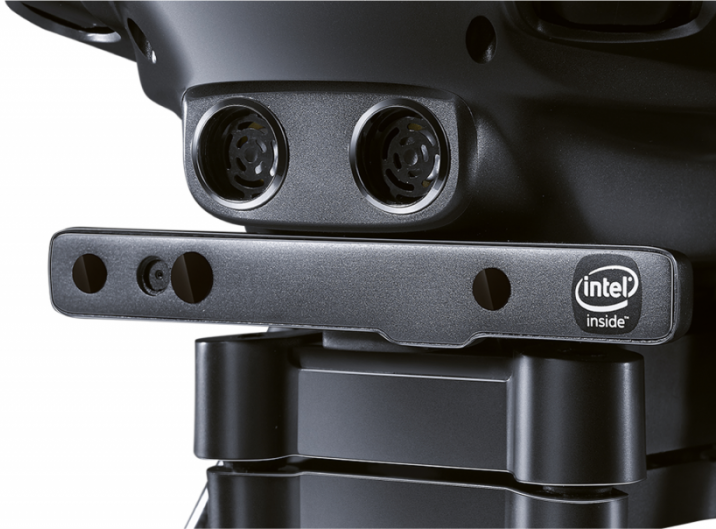
\includegraphics[width=0.35\linewidth]{images/yuneec_closeup.png}
  	\label{subfig:yuneec_closeup}
  }
  \caption{
    (a) Le multi-rotor Yuneec Typhoon H (b) La caméra stéréo infrarouge IntelRealsense augmentée d'un sonar pour détecter les échecs de perception.
  }
  \label{fig:yuneec}
\end{figure}

Dans le contexte des micro-véhicules aériens, il arrive parfois que l'on veuille miniaturiser et simplifier le système à un point où il serait désirable d'avoir un système monoculaire au lieu de stéréo. Tel que mentionné dans la section \ref{subsec:reconstruction} il est possible de mettre à l'échelle une carte 3D construite monoculairement au moyen d'une source d'information métrique secondaire tel qu'une centrale inertielle \citep{muratal2017vimonoslam}. Par contre, pour que cette carte soit utilisable pour la navigation, elle doit être construire de façon à pouvoir représenter les surfaces des obstacles. \cite{Yang2017} proposent de profiter de l'exactitude d'un système d'odométrie visuoinertiel pour construire des cartes de profondeur au moyen de résolution stéréo par mouvement. En d'autres mots, au lieu d'avoir deux caméras pour la triangulation de points, nous avons une seule caméra qui se déplace dans l'espace pour la triangulation.

\section{Systèmes actifs}

Une autre façon de compenser pour les lacunes de la vision stéréo est d'utiliser la vision active, 

\subsection{Time-of-flight}

\subsection{Projection laser}
